\documentclass{article}

\usepackage{amsmath}
\usepackage{amsthm}
\usepackage{tikz}
\usetikzlibrary{shapes,positioning,arrows}
\tikzset {
wissen/.style={shape=rectangle,draw},
phase/.style={shape=ellipse,draw,fill=white}
}

\newcommand{\defined}[1]{{\bf #1}}
\newcommand{\var}[1]{{\em #1}}

\theoremstyle{definition}
\newtheorem{definition}{Definition}

\theoremstyle{remark}
\newtheorem{remark}{Bemerkung}
\begin{document}
\tableofcontents

\section{Grundlagen}
\begin{definition}
Anwender, aktiver Anwender\\
Die Benutzer des Programmes werden im folgenden als \defined{Anwender} bezeichnet.
  Im Folgendenden bezeichnen \var{A}, \var{B} zwei Anwender, die das Programm 
verwenden.\\
  Aus technischen Gr\"unden wird einer der beiden Anwender als 
\defined{aktiver Anwender} bezeichnet und der andere der beiden Anwender als
\defined{passiver Anwender}. Der aktive Anwender ist in der Lage, den Ablauf
eines Protokolles zu initiieren, w\"ahrend der passive Anwender auf die 
Initiierung eines Protokolles durch den aktiven Anwender wartet. Es sei im
folgenden \var{A} der aktive Anwender und \var{B} der passive Anwender.
\end{definition}

\begin{definition}
Wissen, Wissen eines Anwenders, gemeinsames Wissen.\\
Wenn \var{A} ein Anwender ist, so bezeichnen Ausdr\"ucke der Form 
\defined{\var{A.x}} f\"ur Variablen \var{x} \defined{Wissen des Anwenders}. 
Auf das Wissen des Anwenders kann nur der Anwender selbst zugreifen.
Das Wissen eines Anwenders kann \defined{\var{A.x} = \var{e}} erweitert werden.\\
Wenn ein Ausdruck \var{e} als \defined{gemeinsames Wissen c} bezeichnet wird, 
so ist dies \"aquivalent dazu, dass f\"ur alle beteiligten Anwender 
A \var{A.c} = \var{e} ist.
\end{definition}

\begin{definition}
Protokoll.\\
Wir bezeichnen im Folgenden eine Sequenz von Nachrichtenaustauschen zwischen
zwei Anwendern als \defined{Protokoll}
\end{definition}

\begin{definition}
Zwei-Parteien-Berechnung, private Zwei-Parteien-Berechnung, Eingabe, Ausgabe\\
Gegeben zwei Anwender \var{A}, \var{B} mit Wissen \var{A.i} und \var{B.i}
und eine Funktion \var{f}, dann wird ein Protokoll als
\defined{Zwei-Parteien-Berechnung} von Wissen j bezeichnet, wenn nach 
Ausf\"uhrung des Protokolls  \(A.j = f(A.i, B.i) \wedge B.j = f(A.i, B.i) \)
gilt. Wir bezeichnen i als \defined{Eingabe} des Protokolles der Anwender
und j als \defined{Ausgabe} des Protokolles.\\
Wenn ausserdem gilt, dass \var{A} nur \var{A.j} als Wissen ueber \var{B.i}
erh\"alt und dass \var{B} nur \var{B.j} als Wissen ueber \var{A.i} erh\"alt,
dann bezeichnen wir das Zwei-Parteien-Protokoll als \defined{privates
Zwei-Parteien-Protokoll}.
\end{definition}

\begin{remark}
Wenn ein Zwei-Parteien-Protokoll eine Funktion \var{f} berechnen soll,
die Eingaben \var{X} zus\"atzlich zum Wissen der Benutzer erfordert, 
kann dies durch Definition einer Funktion \var{f'(i, j) = f(x, i, j)}
erreicht werden. Dadurch k\"onnen beispielsweise gemeinsames Wissen oder
zuvor festzulegende Parameter genutzt werden. Damit ist die Definition 4
ausreichend, um beliebige Funktionen zu beschreiben.
\end{remark}

\begin{definition}
Phase, private Phase\\
Wir bezeichnen im Folgenden einen Schritt der Anwendung als \defined{Phase}.
Eine Phase erfordert ein gewisses \defined{Vorwissen} der beteiligten Anwender
und garantiert dann, dass nach Ausfuehren der Phase ein gewisses anderes
Wissen erlangt wird. Rein technisch ist eine Phase also nur ein Synonym f\"ur 
eine Funktion auf dem Wissen der Anwender. Damit ergibt sich jedoch, dass
sich auch die Phasen klassifizieren lassen. Eine \defined{private Phase} ist
somit eine Phase, bei der die beteiligten Anwender \"uber das Vorwissen der
anderen beteiligten Anwender nur das Wissen erhalten, dass sie aus dem 
durch die Phase berechneten Wissen schlussfolgern k\"onnen. Eine
\defined{getrennte Phase} ist eine Phase, welche keine Kommunikation zwischen
den Anwendern erfordert.\\
Im folgenden werden wir Bilder von Phasen darstellen. In diesen Bildern werden
im Allgemeinen nur zwei Anwender dargestellt sein. In diesem Bild ist das
Vorwissen und das erhaltene Wissen der Anwender als Rechtecke dargestellt
werden. Das Wissen der Anwender ist durch eine vertikale Linie getrennt und 
der linke Anwender wird ,,Alice'' genannt, w\"ahrend der rechte Anwender Bob
genannt wird. Die Ausf\"uhrung einer Phase wird als Kreis zwischen beiden 
Anwendern dargestellt werden, Pfeile von einem Wissens-Rechteck in 
einen solchen Phasen-Kreis sollen andeuten, dass die Phase dieses Wissen
verwendet und Pfeile von einem solchen Phasen-Kreis zu einem Wissensrechteck
sollen andeuten, dass die Phase dieses Wissen erzeugt. Falls eine Phase 
getrennt ist, wird der bzw die Phasenkreise vollst\"andig in die H\"alfte eines
Anwenders gezeichnet, andernfalls wird der Phasenkreis auf der gestrichelten
Trennlinie gezeichnet werden. Eine einfache \"Ubertragung von Wissen wird
dargestellt als Pfeil von einem Wissens-Recheckt \"uber die gestrichelte
Linie zu einem anderen Wissens-Rechteck. (vgl auch Figure ~\ref{fig:phaseExample})
\end{definition}

\begin{figure}
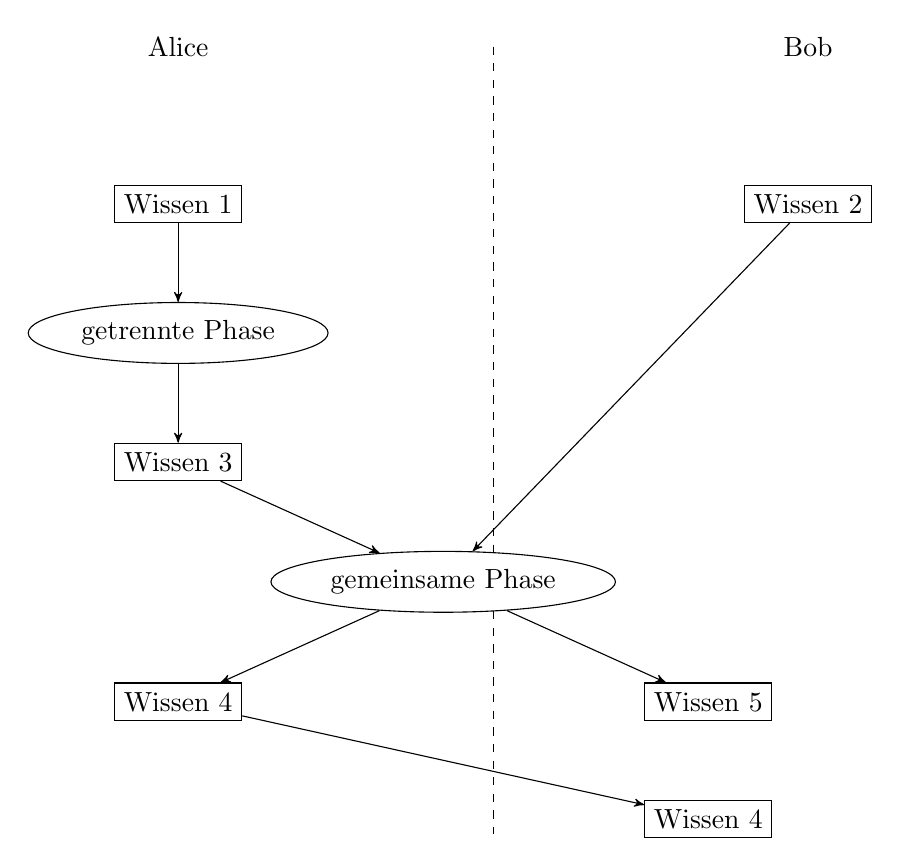
\begin{tikzpicture}
[>=stealth']
\draw (0, 0) node {Alice};
\draw (8, 0) node {Bob};
\draw[dashed] (4, 0) -- (4, -10);
\node (w1) at (0, -2) [wissen] {Wissen 1};
\node (w2) at (8, -2) [wissen] {Wissen 2};
\node[phase] (p1) [below=of w1] {getrennte Phase};
\node[wissen] (w3) [below=of p1] {Wissen 3};
\node[phase] (p2) [below right=of w3] {gemeinsame Phase};
\node[wissen] (w4) [below left=of p2] {Wissen 4};
\node[wissen] (w5) [below right=of p2] {Wissen 5};
\node[wissen] (w6) [below=of w5] {Wissen 4};
\draw[->] (w1) -- (p1);
\draw[->] (p1) -- (w3);
\draw[->] (w3) -- (p2);
\draw[->] (w2) -- (p2);
\draw[->] (p2) -- (w4);
\draw[->] (p2) -- (w5);
\draw[->] (w4) -- (w6);
\end{tikzpicture}
\caption{Phasenbild: Alice mit Phase alleine, beide mit gemeinsamer Phase, Alice sendet Wissen an Bob.}
\label{fig:phaseExample}
\end{figure}
\section{Design der Anwendung}
Es wird nun die Anwendung designed. Hierzu wird r\"uckw\"arts vorgegangen, d.h.,
wir betrachten zuerst, welche Ausgabe die Anwendung produzieren soll und 
betrachten dann Alternativen, diese Ausgabe zu erzeugen. Dadurch ergeben sich
dann weitere ben\"otigte Eingaben f\"ur diese Schlussphase der Anwendung, die
dann rekursiv behandelt werden k\"onnen, bis als Eingabe nur noch die 
vorklassifizierten E-Mails und andere Anwendereingaben \"ubrig bleiben.
An diesem Punkt ist die Anwendung dann fertig designed.\\
Um zu rekapitulieren, die Vision der Anwendung ist:,,Ich habe eine Menge von
vorklassifizierten E-Mails und kenne einen Anwender, der ebenfalls eine Menge
von vorklassifizierten E-Mails hat und will gemeinsam mit diesem einen 
Klassifikator fuer Spam und Nicht-Spam berechnen. Dabei will ich jedoch, dass
er \"uber meine E-Mails nur soviel lernt, wie ich will und wie der Klassifikator
preisgibt.''. Wenn wir diese Vision als Phasendiagramm formulieren, ergibt sich 
Abbildung ~\ref{fig:vision}.\\
\begin{figure}
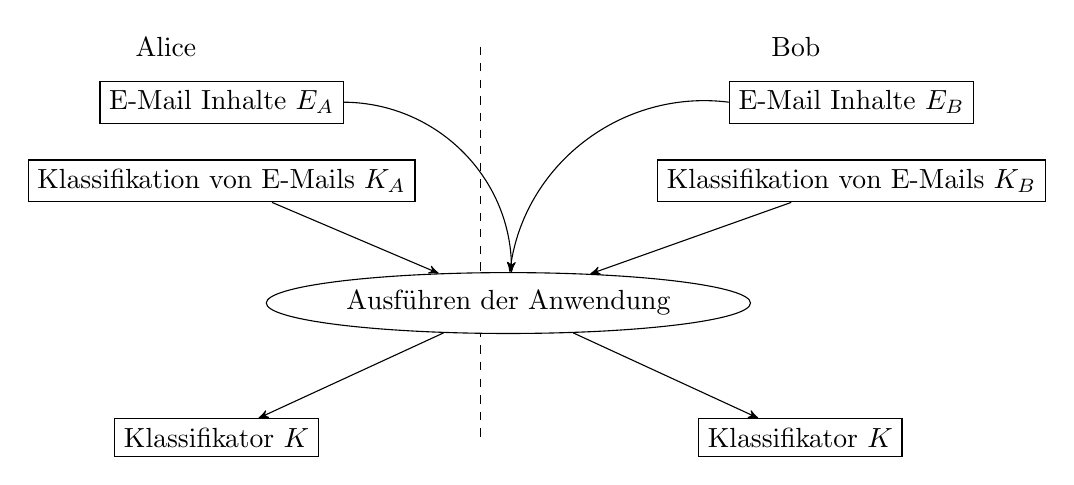
\begin{tikzpicture}
[>=stealth']
\node (alice) at (0, 0) {Alice};
\node (bob) at (8, 0) {Bob};
\draw[dashed] (4, 0) -- (4, -5);
\node[wissen] (emails alice) [below right of=alice] {E-Mail Inhalte \(E_A\)};
\node[wissen] (emails bob) [below right of=bob] {E-Mail Inhalte \(E_B\)};
\node[wissen] (klassifizierung von alices mails) [below of=emails alice] {Klassifikation von E-Mails \(K_A\)};
\node[wissen] (klassifizierung von bobs mails) [below of=emails bob] {Klassifikation von E-Mails \(K_B\)};
\node[phase] (anwendung) [below right=of klassifizierung von alices mails,xshift=-2cm] {Ausf\"uhren der Anwendung};
\node[wissen] (klassifikator alice) [below left of=anwendung,xshift=-3cm,yshift=-1cm] {Klassifikator \(K\)};
\node[wissen] (klassifikator bob) [below right of=anwendung,xshift=3cm,yshift=-1cm] {Klassifikator \(K\)};

\draw[->] (emails alice.east) to [bend left=45] (anwendung);
\draw[->] (klassifizierung von alices mails) to (anwendung);
\draw[->] (emails bob.west) to [bend right=45] (anwendung);
\draw[->] (klassifizierung von bobs mails) to (anwendung);
\draw[->] (anwendung) to (klassifikator alice);
\draw[->] (anwendung) to (klassifikator bob);
\end{tikzpicture}
\caption{Phasendiagramm der Anwendung: Beide haben Inhalte und Vorklassifizierungen und wollen einen Klassifikator}
\label{fig:vision}
\end{figure}

\subsection{Erstellung des Klassifikators}
\subsubsection{Verwenden eines nicht verteilten Klassifikators}
Um das Vorgehen zu verstehen und der Vollst\"andigkeit halber wird die
M\"oglichkeit aufgef\"uhrt, den Klassifikator nicht verteilt
zu berechnen. Dazu wird das vollst\"andige Wissen ausgetauscht und 
dann lokal der Klassifikator berechnet. Dies ist in Abbildung 
~\ref{fig:local_computation_phase_diagram} dargestellt. Es ist deutlich
zu erkennen, dass die Eingabe der Anwendung die Klassifikation und die E-Mails
des Anwenders sind und dass die Ausgabe des Protokolls ein Klassifikator ist.
Wenn beide Anwender sich an das Protokoll halten, ist dies sogar der gleiche
Klassifikator f\"ur beide, sodass die Vision durch diese Implementierung
erf\"ullt wird.\\
Es gibt in dieser Vorgehensweise keinerlei Geheimhaltung, da alle Eingaben der 
Anwender an alle anderen Anwender \"ubertragen werden. \\
Die Implementierung dieses Szenarios ist einfach, da Implementierungen f\"ur
viele Lernverfahren zu finden sind und die initiale \"Ubertragung einfach
zu implementieren ist. 
\begin{figure}
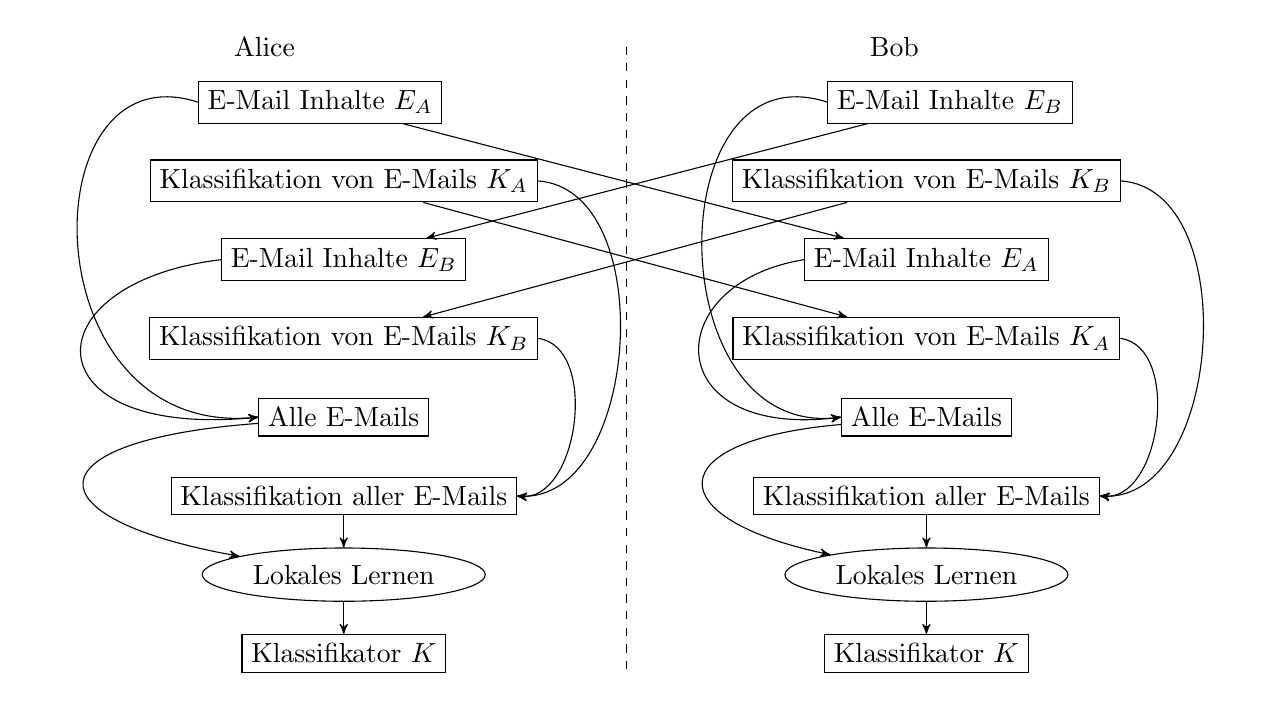
\begin{tikzpicture}
[>=stealth',node distance=1cm]
\node (alice) at (0,0) {Alice};
\node (bob) at (8,0) {Bob};
\draw[dashed] (4.6,0) -- (4.6, -8);
\node[wissen] (emails alice) [below right of=alice] {E-Mail Inhalte \(E_A\)};
\node[wissen] (emails bob) [below right of=bob] {E-Mail Inhalte \(E_B\)};
\node[wissen] (klassifizierung von alices mails) [below of=emails alice,xshift=0.3cm] {Klassifikation von E-Mails \(K_A\)};
\node[wissen] (klassifizierung von bobs mails) [below of=emails bob,xshift=-0.3cm] {Klassifikation von E-Mails \(K_B\)};
\node[wissen] (emails alice bei bob) [below of=klassifizierung von bobs mails] {E-Mail Inhalte \(E_A\) };
\node[wissen] (klassifizierung von alices mails bei bob) [below of=emails alice bei bob] {Klassifikation von E-Mails \(K_A\)};
\node[wissen] (emails bob bei alice) [below of=klassifizierung von alices mails] {E-Mail Inhalte \(E_B\) };
\node[wissen] (klassifizierung von bobs mails bei alice)  [below of=emails bob bei alice] {Klassifikation von E-Mails \(K_B\)};
\node[wissen] (alle mails bei alice) [below of=klassifizierung von bobs mails bei alice] {Alle E-Mails};
\node[wissen] (alle mails bei bob) [below of=klassifizierung von alices mails bei bob] {Alle E-Mails};
\node[wissen] (klassifizierung aller mails bei alice) [below of=alle mails bei alice] {Klassifikation aller E-Mails};
\node[wissen] (klassifizierung aller mails bei bob) [below of=alle mails bei bob] {Klassifikation aller E-Mails};
\node[phase] (alice lokal) [below of=klassifizierung aller mails bei alice] {Lokales Lernen};
\node[phase] (bob lokal) [below of=klassifizierung aller mails bei bob] {Lokales Lernen};
\node[wissen] (klassifikator alice) [below of=alice lokal] {Klassifikator \(K\)};
\node[wissen] (klassifikator bob) [below of=bob lokal] {Klassifikator \(K\)};

\draw[->] (emails alice) to (emails alice bei bob);
\draw[->] (emails bob) to (emails bob bei alice);
\draw[->] (klassifizierung von alices mails) to (klassifizierung von alices mails bei bob);
\draw[->] (klassifizierung von bobs mails) to (klassifizierung von bobs mails bei alice);
\draw[->] (emails alice.west) .. controls (-3,0) and (-3,-5) ..(alle mails bei alice.west);
\draw[->] (emails bob bei alice.west) .. controls(-3, -3) and (-3, -5) .. (alle mails bei alice.west);
\draw[->] (emails bob.west) .. controls (5, 0) and (5, -5) .. (alle mails bei bob.west);
\draw[->] (emails alice bei bob.west) .. controls(5, -3) and (5, -5) .. (alle mails bei bob.west);
\draw[->] (klassifizierung von bobs mails bei alice) to [bend left=90] (klassifizierung aller mails bei alice);
\draw[->] (klassifizierung von alices mails) to [bend left=90] (klassifizierung aller mails bei alice);
\draw[->] (klassifizierung von bobs mails.east) to [bend left=90] (klassifizierung aller mails bei bob.east);
\draw[->] (klassifizierung von alices mails bei bob.east) to [bend left=90] (klassifizierung aller mails bei bob.east);

\draw[->] (klassifizierung aller mails bei alice) to (alice lokal);
\draw[->] (alle mails bei alice) .. controls (-3, -5) and (-3, -6) .. (alice lokal);

\draw[->] (klassifizierung aller mails bei bob) to (bob lokal);
\draw[->] (alle mails bei bob) .. controls (5, -5) and (5, -6) .. (bob lokal);

\draw[->] (alice lokal) to (klassifikator alice);
\draw[->] (bob lokal) to (klassifikator bob);
\end{tikzpicture}
\caption{Lokale Berechnung der Klassifikatoren}
\label{fig:local_computation_phase_diagram}
\end{figure}

\subsubsection{Verwenden von Entscheidungsb\"aumen}
\begin{definition} Entscheidungsbaum\\
Generell lassen sich Entscheidungsb\"aume wie folgt definieren: Es gibt eine
Menge \(A\) von diskreten Attributen \({A_1, A_2, \dots, A_n}\) mit Werten
\(values(A_i) = {v^1_i, v^2_i, \dots, v^w_i}\) und es gibt zu erkennde
Klassen \(K = {K_1, K_2, \dots, K_k}\). Es bezeichne im Folgenden desweiteren
\(Values = \bigcup_{A_i} values(A_i)\) die Menge aller m\"oglichen 
Attributwerte (dies vereinfacht einige Definitionen, auch wenn 
einige Typen etwas ungenauer werden).
Dann kann die Menge \(T\) von Entscheidungsb\"aumen induktiv definiert werden 
als:
\( T = (A \times Values \mapsto T) \cup K\)\\
Ein Entscheidungsbaum klassifiziert eine Abbildung der Attribute auf Werte.
Dieser klassifizierungsvorgang ist induktiv definiert. Wenn der
zu klassifizierende Kandidat mit \(s : A \mapsto Values\)
bezeichnet wird, dann ergibt sich als Auswertungsfunktion
\(evaluate : (A \mapsto Values) \times T \mapsto K\):

\begin{align}
evaluate(s, (A_i, f)) &=& evaluate(s, f(s(A_i)))\\
evaluate(s, K_i) &=& K_i
\end{align}
\end{definition}

Verbal beschrieben besteht ein Entscheidungsbaum also aus Bl\"attern,
die aussagen, dass alle zu klassifizierenden Objekte, die dieses Blatt 
,,erreichen'' zu dieser bestimmten Klasse geh\"oren und \"Asten, 
die mit einem Attribut annotiert sind und zu jedem m\"oglichen 
Wert des Attributes einen Unterbaum haben. Bei der Klassifizierung 
werden dann die \"Aste entsprechend der Attributwerte des zu 
klassifizierenden Objektes traversiert, bis ein Blatt erreicht 
wird und die Klassifizierung abgeschlossen ist.\\
Wenn wir beispielsweise annehmen, dass wir uns bei der Spamerkennung dadrauf
geeinigt haben, dass wir als Attribute verwenden, ob die Worte "Foo" bzw
"Bar" oft oder selten vorkommen, dann w\"urden die
E-Mail-Datenbanken transformiert werden zu einem Vektor von Abbildungen
von Foo und Bar auf oft oder selten:\\
\begin{tabular}{c c}
Vorkommnisse Foo & Vorkommnisse Bar \\
Oft & Oft \\
Selten & Oft \\
Selten & Selten \\
\end{tabular}
Ein m\"oglicher Entscheidungsbaum ist in Abbildung ~\ref{fig:decision_tree_example} 
dargestellt, der die Mails in Spam und Nicht Spam klassifiziert. Es ist hier ein
Baum aufgezeichnet, der prinzipiell nur Mails als ,,Nicht Spam'' klassifiziert,
wenn sie oft Foo und Bar enthalten. In der Grafik ist zudem illustriert, welche 
Knoten und damit welche Kanten bei der Auswertung betrachtet wurden.
\begin{figure}
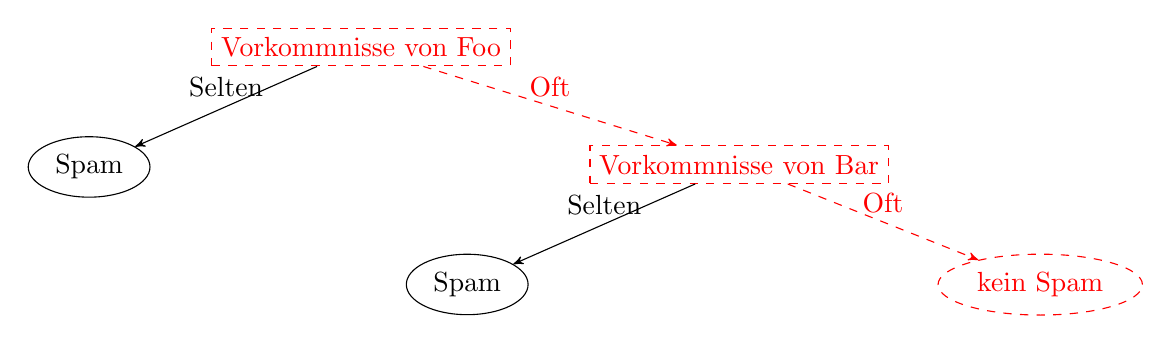
\begin{tikzpicture}
[branch/.style={shape=rectangle,draw},
 leaf/.style={shape=ellipse,draw},>=stealth']
\node[branch] (foo) [color=red,dashed] {Vorkommnisse von Foo};
\node[leaf] (spam1) [below left=of foo] {Spam};
\node[branch] (bar) [color=red,dashed] [below right=of foo] {Vorkommnisse von Bar};
\node[leaf] (spam2) [below left=of bar] {Spam};
\node[leaf] (spam3) [color=red,dashed,below right=of bar] {kein Spam};

\draw[->] (foo) to node[above]{Selten} (spam1);
\draw[->,dashed,color=red] (foo) to node[above] {Oft} (bar);
\draw[->] (bar) to node[above] {Selten} (spam2);
\draw[->,dashed,color=red] (bar) to node[above] {Oft} (spam3);
\end{tikzpicture}
\caption{M\"oglicher Entscheidungsbaum, Klassifizierung von 
,,Foo \(\rightarrow\) Oft, Bar \(\rightarrow\) Oft''}
\label{fig:decision_tree_example}
\end{figure}

Ausgehend von dem ausgeteilten Paper gibt es ein privates 2 Parteien Protokoll,
welches ein Lernverfahren, den ID3-Algorithmus, durchf\"uhrt. Der ID3-Algorithmus
ist ein heuristisches Verfahren, um aus einer Menge vorklassifizierte Zuordnungen
einen Entscheidungsbaum zu produzieren. Damit kann man das in Abbildung ~\ref{fig:phase:id3}
gezeigte Phasendiagramm aufstellen. Es muss somit festgelegt werden, wie die 
Attribute entstehen und wie die E-Mails diskretisiert werden m\"ussen, um dann den
ID3-Algorithmus verteilt und privat auszuf\"uhren und somit den Klassifikator zu
berechnen.
\(<TODO| ID3 zusammenfassen, verteilung erlaeutern?>\)
\(<TODO| Bewertung>\)
\begin{figure}
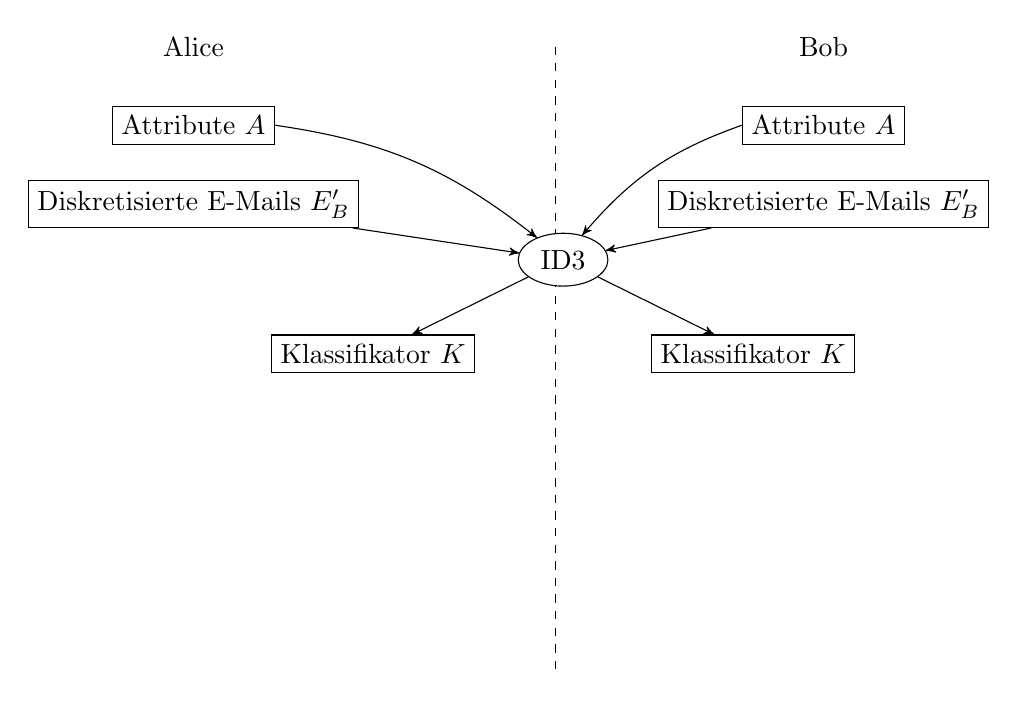
\begin{tikzpicture}
[>=stealth',node distance=1cm]
\node (alice) at (0,0) {Alice};
\node (bob) at (8,0) {Bob};
\draw[dashed] (4.6,0) -- (4.6, -8);
\node[wissen] (alice attribute) [below of=alice] {Attribute \(A\)};
\node[wissen] (alice emails) [below of=alice attribute] {Diskretisierte E-Mails \(E'_B\)};
\node[wissen] (bob attribute) [below of=bob] {Attribute \(A\)};
\node[wissen] (bob emails) [below of=bob attribute] {Diskretisierte E-Mails \(E'_B\)};
\node[phase] (ID3) [below left of=bob emails,xshift=-2.6cm] {ID3};
\node[wissen] (alice klassifikator) [below left=of ID3] {Klassifikator \(K\)};
\node[wissen] (bob klassifikator) [below right=of ID3] {Klassifikator \(K\)};

\draw[->] (alice attribute.east) to [bend left=15] (ID3);
\draw[->] (bob attribute.west) to [bend right=15] (ID3);
\draw[->] (alice emails) to (ID3);
\draw[->] (bob emails) to (ID3);
\draw[->] (ID3) to (alice klassifikator);
\draw[->] (ID3) to (bob klassifikator);
\end{tikzpicture}
\caption{Phasendiagramm bei Verwendung von Entscheidungsb\"aumen und dem ID3-Algorithmus}
\label{fig:phase:id3}
\end{figure}

\subsection{Festlegen der Attribute, Transformieren der E-Mails}
Da wir keine Attributsvektoren als Eingaben haben, sondern nur Texte ist es
notwendig, M\"oglichkeiten der Transformation zu untersuchen. 

\subsubsection{Berechnung einer Wahrscheinlichkeit und Diskretisierung}
Eine gute M\"oglichkeit, derartige Vektoren zu erzeugen ist es, Vorkommnisse
irgendeiner Form zu z\"ahlen, in Relation mit einer Gesamtanzahl zu setzen und 
danach dieses Verh\"ahltnis zu diskretisieren. Damit gibt es zwei weitere 
Unterprobleme: Wie bekommen wir diese Wahrscheinlichkeit, und wie diskretisieren
wir sie?\\
Prinzipiell gibt es f\"ur die Diskretisierung zwei grosse Fragen: Wieviele 
Wertebereiche verwenden wir und wer bestimmt die Schwellwerte zwischen den
Wertebereichen? Dies ist eine Entscheidung, die der Kunde treffen muss. Es muss
hier bedacht werden, dass zuwenige Wertebereiche sehr grob sind (bei 
nur einem Wertebereich gibt es nur die Aussage, dass das Attribut betrachtet
wurde, bei nur zwei Wertebereichen gibt es nur eine binaere Aussage) und dass
zuviele Wertebereiche Probleme haben zu abstrahieren (Bei
1024 Wertebereichen abstrahiert man kaum noch von den eigentlichen
Daten, weil (etwas dramatisiert) fast jeder Datenpunkt seinen 
eigenen Wertebereich hat. Damit w\"are der Klassifikator dann praktisch
nur auswendig gelerntes Wissen).\\
F\"ur das Festlegen der Schwellwerte gibt es mehr Freiraum. Die erste Variante
besteht darin, {\em den Nutzer die Werte eingeben zu lassen}. Dies erfordert dann
eine Syncronisierung der Werte beider Anwender, ist dann jedoch maximal
flexibel, da der Anwender alle M\"oglichkeiten hat, diese Schwellwerte zu 
bestimmen (neuartige Mustererkennungsalgorithmen, stundenlanges tunen der
Werte).\\
Die zweite Variante besteht darin, dass {\em das Programm diese Werte selbst 
bestimmt}. Eine M\"oglichkeit hierzu besteht darin, das Histogramm der 
Wahrscheinlichkeitsverteilung zu betrachten und dann die Werte so zu platizeren,
dass die Integrale in den Teilintervallen m\"oglichst gleich gross sind. Das
sollte dann die Information der einzelnen diskreten Werte maximieren. Der
Vorteil hier besteht darin, dass dann die Werte nicht vom Anwender eingegeben
werden m\"ussen. Der Nachteil besteht darin, dass so keine M\"oglichkeit besteht,
einen anderen, besseren Algorithmus zu verwenden. (Man beachte auch, dass man
mit Variante 1 implementieren kann und dann Variante 2 durch Variante 1
implementiert mitliefern kann).\\
Fuer die Syncronisierung der Werte kann man praktisch beliebige Funktionen
verwenden, die zwei Sequenzen von reellen Zahlen auf eine Sequenz reeller
Zahlen abbildet. Damit ist es etwas aufw\"andig, alle M\"oglichkeiten
aufzuz\"ahlen. Eine Variante, die sich jedoch anbietet, ist das punktweise
Arithmetische Mittel zu bilden, da hier die von beiden Nutzern verwendeten
Schwellwerte zu gleichen Teilen beruecksichtigt werden. Zudem ist die
Implementierung denkbar einfach, da der punktweise Mittelwert zweier 
streng monoton steigender Folgen streng monoton steigend ist und somit 
der punktweise Mittelwert von zwei Vektoren von Hysteresepunkten wieder
ein Vektor von Hysteresepunkten ist. \\
F\"ur die Berechnung von Wahrscheinlichkeiten gibt es ebenfalls mehrere
M\"oglichkeiten. Die erste Klasse von Berechnungen drehen sich alle um 
die Anzahl der Vorkomnisse von Wortmengen. Es wird hierzu eine Menge von Mengen
von Strings definiert und f\"ur jede dieser Stringmengen untersucht, welcher
Prozentsatz der Worte in einer E-Mail in jeder dieser Stringmengen liegt.
Wenn der Inhalt einer E-Mail beispielsweise "Foo Bar Baz" ist, und die
Wortmengen \(\{"Foo", "Bar"\}\), \(\{"Bar", "Baz"\}\), \(\{"Baz"\}\), dann sind
die Vorkommnisse \(\frac{2}{3}, \frac{2}{3}, \frac{1}{3}\). (Dies ist eine
Generalisierung des vorherigen Ansatzes der Wortliste. Die Wortliste vom
letzten Mal ist im Endeffekt eine solche Stringmenge, in der alle Mengen
nur ein einzelnes Element enthalten).
\(<TODO|Bewertung>\)
\(<TODO|Phasendiagramm>\)

\end{document}
